\chapter{Calunium assembly}

\section{Introduction}

The Calunium microcontroller development board is intended to be a
flexible system for both development and embedded use. As such it has
various hardware options and careful attention must be paid to
assembling it for optimum performance. Parts which are not needed are
omitted to lower power consumption (\eg, power LED, USB controller).

\section{Calunium version 2.0 and version 2.1}

\begin{figure}
  \centering
  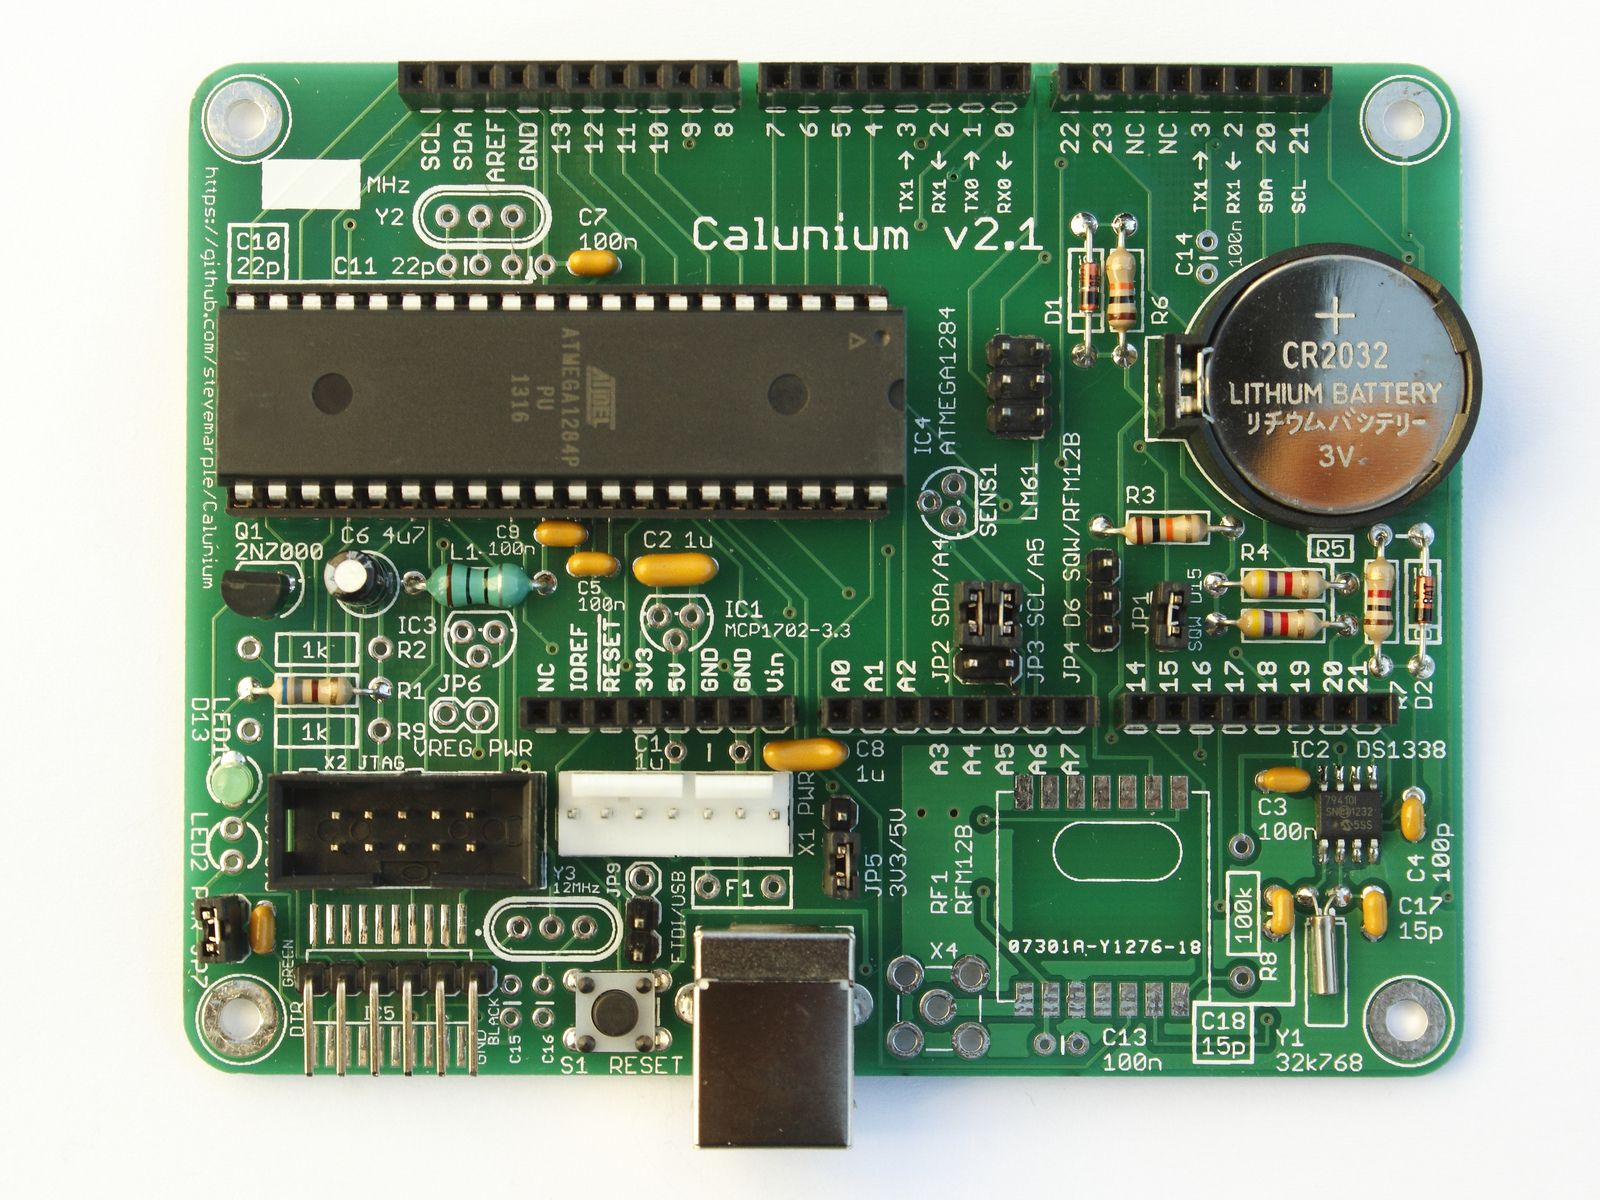
\includegraphics[keepaspectratio,width=\textwidth]{%
    images/calunium-v2-1}
  \caption[Completed Calunium v2.1]{%
    Completed Calunium v2.1. \photoCredit{Steve Marple}{\ccBySaTwo}{%
      http://www.flickr.com/photos/stevemarple/10786865096/}}
  \label{fig:calunium-version-2.1}
\end{figure}

\subsection{Order of assembly}

Fit components in order:
\begin{buildorder}
\item IC2. The standard real-time clock is the MicroChip MCP90410 but
  MicroChip MCP79411 or MCP79412 can be used without any other
  changes.
  It is also possible to fit the Maxim DS1338-33 real-time clock,
  but see below for changes.
\item Y1 (\kHz{32.768}).
\item R1, fit a \ohm{680} resistor. Ignore the \kohm{1} marking; a
  lower value resistor is used to enable the green LED to be seen
  more clearly in daylight.
\item R7 (\kohm{1}). Do not fit if using the DS1338-33 real-time
  clock. Instead link between R7 and D2 at the end nearest the \rtc\
  battery, as indicated by the white line on the silkscreen. The wire
  will bypass both R7 and D2 which are not required for the DS1338-33.
\item R4, R5 (\kohm{4.7}).
\item R3, R6 (\kohm{10}).
\item L1 (\uH{10}).
\item 40~pin socket for IC4.
\item C4 (\pF{100}).
\item C3, C5, C7, C9, C12 (\nF{100}).
\item C2, C8 (\uF{1}).
\item D1, D2 (BAT85). Do not fit D2 if using the DS1338-33 real-time clock.
\item LED1 (green LED). The cathode is nearest LED2, see
  figure~\ref{fig:calunium-led-orientation}.
\item C6 (\uF{4.7}).
\item ICSP header ($2 \times 3$ jumper block). See
  \figurename~\ref{fig:icsp-header}.
\item JP2 and JP3. Fit as combined $2 \times 3$ jumper block.
\item JP1, JP7 ($1 \times 2$ jumper).
\item JP4, JP5 ($1 \times 5$ jumper).
\item X5 ($1 \times 6$ right-angle or vertical header for UART0).
\item S1 (reset switch).
\item Arduino headers. \todo[Add description]
\item C17, C18 (\pF{15}). Do not fit if using DS1338-33 \rtc. For
  Calunium verion 2.0 the capacitors must be fitted on the reverse
  side of the board (see \figurename~\ref{fig:calunium-rtc-caps-hack}
  as no specific mounting holes exist (error caused by using an
  earlier, incorrect datasheet which did not show the load
  capacitors).
\item X1 (Molex power header). Ensure correct orientation, with the
  backplate closest to the Arduino headers.
\item \todo[Add component name] (\rtc\ battery holder).
\item Q1 (2N7000). This item is very sensitive to damage by
  electrostatic discharge!
\item Battery (CR2032). Check that the battery backup pin (3) on the
  \rtc\ measures \volt{3.0}.
\item \todo[Fit shunts to jumpers \ldots]
\end{buildorder}
Do not fit the ATmega1284P microcontroller until after testing the
board power supplies.

\begin{figure}
  \centering
  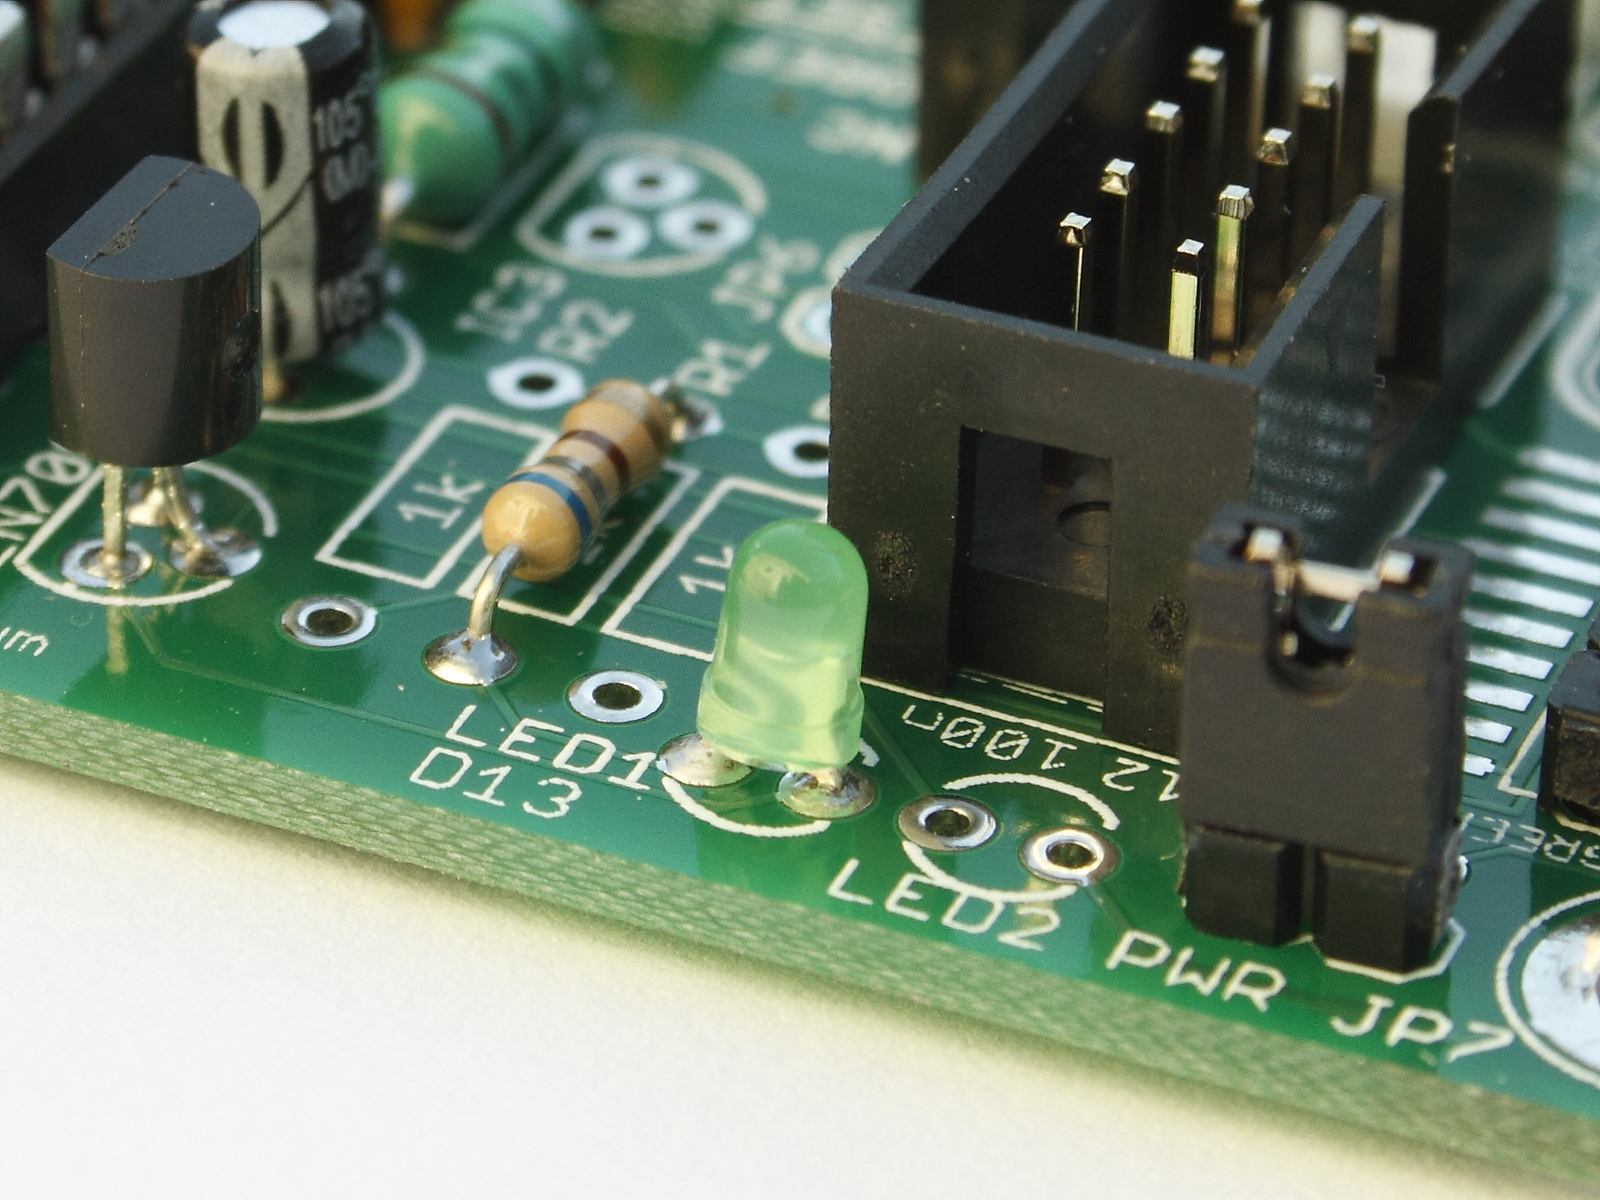
\includegraphics[keepaspectratio,width=10cm]{%
    images/calunium-led-orientation}
  \caption[LED orientation]{\led\ orientation. \photoCredit{%
      Steve Marple}{\ccBySaTwo}{%
      http://www.flickr.com/photos/stevemarple/10786846715/}}
  \label{fig:led-orientation}
\end{figure}
\begin{figure}
  \centering
  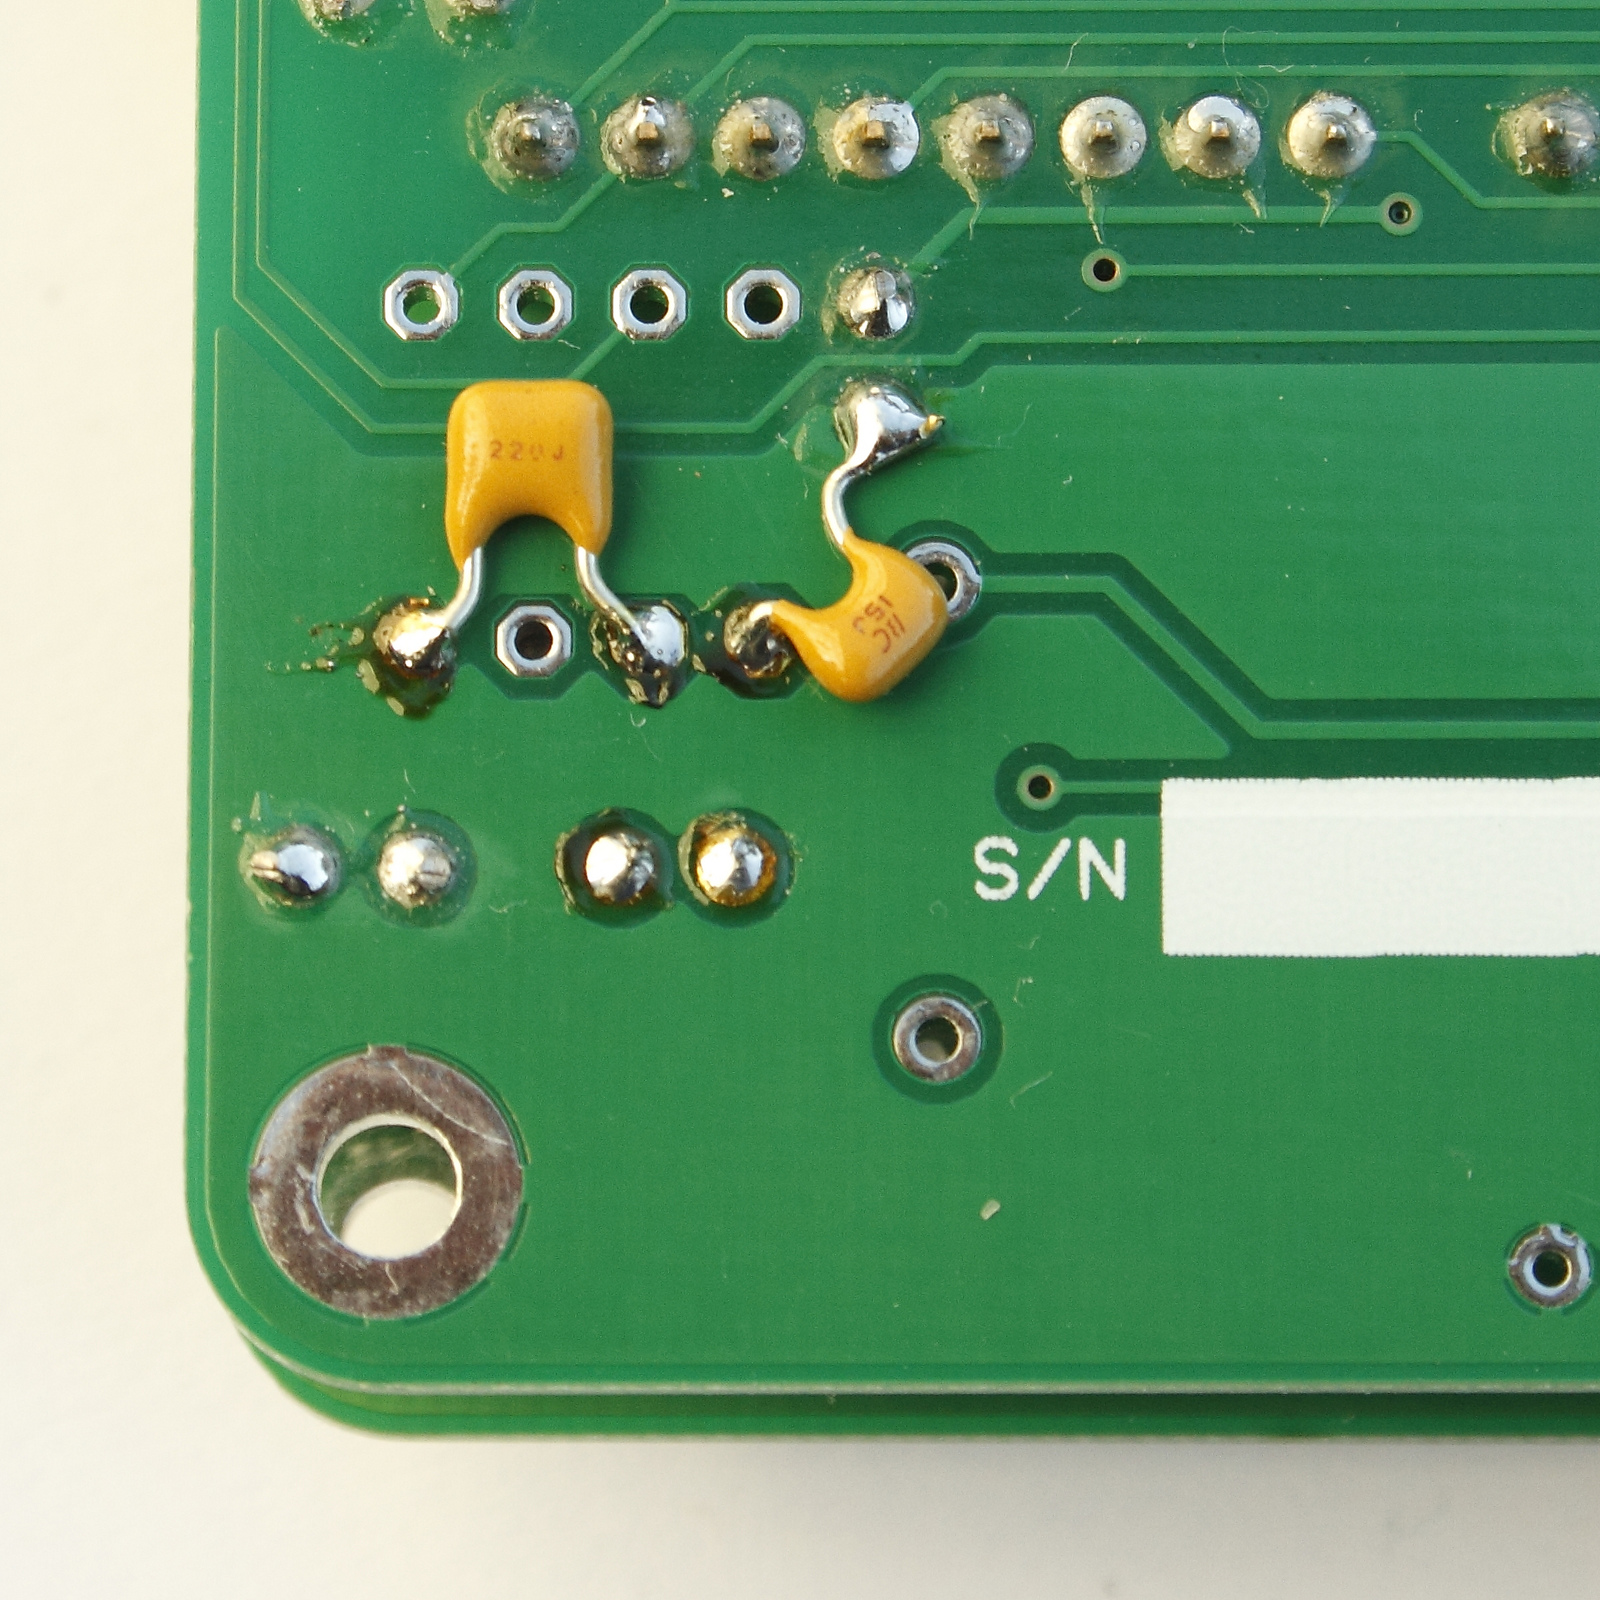
\includegraphics[keepaspectratio,width=10cm]{%
    images/calunium-rtc-caps-hack}
  \caption[Real-time clock load capacitors (Calunium v~2.0)]{%
    Real-time clock load capacitors (Calunium v~2.0). \photoCredit{%
      Steve Marple}{\ccBySaTwo}{%
      http://www.flickr.com/photos/stevemarple/10787041263/}}
  \label{fig:calunium-rtc-caps-hack}
\end{figure}


\begin{landscape}
  \begin{figure}[p]
    \centering
    \includegraphics[keepaspectratio,width=28cm,height=16cm]{%
      ../../hardware/Calunium/hardware/pcb/Calunium_v2/Calunium_v2_sch}  
    \caption{Calunium v.~2.0 circuit diagram.}
    \label{fig:calunium-v2.0-cct-diag}
  \end{figure}
  \begin{figure}[p]
    \centering
    % Use symbolic link for image to avoid a filename with a dot in
    % the main part of the name. This enables the extension to be left
    % off for easy processing with either latex or pdflatex.
    \includegraphics[keepaspectratio,width=28cm,height=16cm]{%
      images/Calunium_v2_1_sch}
    \caption{Calunium v.~2.1 circuit diagram.}
    \label{fig:calunium-v2.1-cct-diag}
  \end{figure}
\end{landscape}

\section{Testing the board}

\section{Programming the firmware}

These instructions assume you are using the Atmel AVR Dragon in \isp\
mode but adapting them to suit your programmer should be
straightforward; see the \filename{avrdude} manual page for further
information.

\subsection{Programming the bootloader}

Power up the Calunium board and connect the programmer. Ensure the
cable is correctly orientated at both ends. The bootloader can be
compiled and programmed simply, as user \piUser: \todo[Check directory]
\begin{Cmd}
  cd /home/pi/xboot
  make clean
  make SHELL=bash calunium_8MHz_RC_ISP.conf.mk program
\end{Cmd}
\todo: ignore lock bit verification errors.

If the bootloader is correctly programmed the green \led\ connected to
D13 on the Calunium \pcb\ should flash at about \Hz{1}.

\subsection{Programming the magnetometer firmware}
Ensure that the shunt marked ``AUTO RST'' is fitted, and that the
shunt marked ``FTDI PWR'' is omitted. Connect the FTDI cable and
identify the USB device file; as user \piUser:
\begin{Cmd}
  dmesg | tail
\end{Cmd}

Look for a line containing text similar to
\begin{Cmd}
  FTDI USB Serial Device converter now attached to ttyUSB0
\end{Cmd}
For the case above the device file \filename{/dev/ttyUSB0}. Now
program the microcontroller using the xboot bootloader. Replace
\filename{/dev/ttyUSB0} with the device file one your system. As user
\piUser:
\begin{Cmd}
  cd /home/pi/AuroraWatchNet/firmware/magnetometer
  avrdude -p atmega1284p -b 38400 -c avr109 -P /dev/ttyUSB0 \textbackslash
      -U flash:w:xrf_rf12-0.10a.bin:r
\end{Cmd}


\helpbox{Whilst it is possible to program the firmware using the AVR
  Dragon alone this approach ensures that the xboot bootloader is
  present and functions correctly, allowing the microcontroller
  firmware to be updated over the radio link.}
